
% Default to the notebook output style

    


% Inherit from the specified cell style.




    
\documentclass[11pt]{article}

    
    
    \usepackage[T1]{fontenc}
    % Nicer default font (+ math font) than Computer Modern for most use cases
    \usepackage{mathpazo}

    % Basic figure setup, for now with no caption control since it's done
    % automatically by Pandoc (which extracts ![](path) syntax from Markdown).
    \usepackage{graphicx}
    % We will generate all images so they have a width \maxwidth. This means
    % that they will get their normal width if they fit onto the page, but
    % are scaled down if they would overflow the margins.
    \makeatletter
    \def\maxwidth{\ifdim\Gin@nat@width>\linewidth\linewidth
    \else\Gin@nat@width\fi}
    \makeatother
    \let\Oldincludegraphics\includegraphics
    % Set max figure width to be 80% of text width, for now hardcoded.
    \renewcommand{\includegraphics}[1]{\Oldincludegraphics[width=.8\maxwidth]{#1}}
    % Ensure that by default, figures have no caption (until we provide a
    % proper Figure object with a Caption API and a way to capture that
    % in the conversion process - todo).
    \usepackage{caption}
    \DeclareCaptionLabelFormat{nolabel}{}
    \captionsetup{labelformat=nolabel}

    \usepackage{adjustbox} % Used to constrain images to a maximum size 
    \usepackage{xcolor} % Allow colors to be defined
    \usepackage{enumerate} % Needed for markdown enumerations to work
    \usepackage{geometry} % Used to adjust the document margins
    \usepackage{amsmath} % Equations
    \usepackage{amssymb} % Equations
    \usepackage{textcomp} % defines textquotesingle
    % Hack from http://tex.stackexchange.com/a/47451/13684:
    \AtBeginDocument{%
        \def\PYZsq{\textquotesingle}% Upright quotes in Pygmentized code
    }
    \usepackage{upquote} % Upright quotes for verbatim code
    \usepackage{eurosym} % defines \euro
    \usepackage[mathletters]{ucs} % Extended unicode (utf-8) support
    \usepackage[utf8x]{inputenc} % Allow utf-8 characters in the tex document
    \usepackage{fancyvrb} % verbatim replacement that allows latex
    \usepackage{grffile} % extends the file name processing of package graphics 
                         % to support a larger range 
    % The hyperref package gives us a pdf with properly built
    % internal navigation ('pdf bookmarks' for the table of contents,
    % internal cross-reference links, web links for URLs, etc.)
    \usepackage{hyperref}
    \usepackage{longtable} % longtable support required by pandoc >1.10
    \usepackage{booktabs}  % table support for pandoc > 1.12.2
    \usepackage[inline]{enumitem} % IRkernel/repr support (it uses the enumerate* environment)
    \usepackage[normalem]{ulem} % ulem is needed to support strikethroughs (\sout)
                                % normalem makes italics be italics, not underlines
    

    
    
    % Colors for the hyperref package
    \definecolor{urlcolor}{rgb}{0,.145,.698}
    \definecolor{linkcolor}{rgb}{.71,0.21,0.01}
    \definecolor{citecolor}{rgb}{.12,.54,.11}

    % ANSI colors
    \definecolor{ansi-black}{HTML}{3E424D}
    \definecolor{ansi-black-intense}{HTML}{282C36}
    \definecolor{ansi-red}{HTML}{E75C58}
    \definecolor{ansi-red-intense}{HTML}{B22B31}
    \definecolor{ansi-green}{HTML}{00A250}
    \definecolor{ansi-green-intense}{HTML}{007427}
    \definecolor{ansi-yellow}{HTML}{DDB62B}
    \definecolor{ansi-yellow-intense}{HTML}{B27D12}
    \definecolor{ansi-blue}{HTML}{208FFB}
    \definecolor{ansi-blue-intense}{HTML}{0065CA}
    \definecolor{ansi-magenta}{HTML}{D160C4}
    \definecolor{ansi-magenta-intense}{HTML}{A03196}
    \definecolor{ansi-cyan}{HTML}{60C6C8}
    \definecolor{ansi-cyan-intense}{HTML}{258F8F}
    \definecolor{ansi-white}{HTML}{C5C1B4}
    \definecolor{ansi-white-intense}{HTML}{A1A6B2}

    % commands and environments needed by pandoc snippets
    % extracted from the output of `pandoc -s`
    \providecommand{\tightlist}{%
      \setlength{\itemsep}{0pt}\setlength{\parskip}{0pt}}
    \DefineVerbatimEnvironment{Highlighting}{Verbatim}{commandchars=\\\{\}}
    % Add ',fontsize=\small' for more characters per line
    \newenvironment{Shaded}{}{}
    \newcommand{\KeywordTok}[1]{\textcolor[rgb]{0.00,0.44,0.13}{\textbf{{#1}}}}
    \newcommand{\DataTypeTok}[1]{\textcolor[rgb]{0.56,0.13,0.00}{{#1}}}
    \newcommand{\DecValTok}[1]{\textcolor[rgb]{0.25,0.63,0.44}{{#1}}}
    \newcommand{\BaseNTok}[1]{\textcolor[rgb]{0.25,0.63,0.44}{{#1}}}
    \newcommand{\FloatTok}[1]{\textcolor[rgb]{0.25,0.63,0.44}{{#1}}}
    \newcommand{\CharTok}[1]{\textcolor[rgb]{0.25,0.44,0.63}{{#1}}}
    \newcommand{\StringTok}[1]{\textcolor[rgb]{0.25,0.44,0.63}{{#1}}}
    \newcommand{\CommentTok}[1]{\textcolor[rgb]{0.38,0.63,0.69}{\textit{{#1}}}}
    \newcommand{\OtherTok}[1]{\textcolor[rgb]{0.00,0.44,0.13}{{#1}}}
    \newcommand{\AlertTok}[1]{\textcolor[rgb]{1.00,0.00,0.00}{\textbf{{#1}}}}
    \newcommand{\FunctionTok}[1]{\textcolor[rgb]{0.02,0.16,0.49}{{#1}}}
    \newcommand{\RegionMarkerTok}[1]{{#1}}
    \newcommand{\ErrorTok}[1]{\textcolor[rgb]{1.00,0.00,0.00}{\textbf{{#1}}}}
    \newcommand{\NormalTok}[1]{{#1}}
    
    % Additional commands for more recent versions of Pandoc
    \newcommand{\ConstantTok}[1]{\textcolor[rgb]{0.53,0.00,0.00}{{#1}}}
    \newcommand{\SpecialCharTok}[1]{\textcolor[rgb]{0.25,0.44,0.63}{{#1}}}
    \newcommand{\VerbatimStringTok}[1]{\textcolor[rgb]{0.25,0.44,0.63}{{#1}}}
    \newcommand{\SpecialStringTok}[1]{\textcolor[rgb]{0.73,0.40,0.53}{{#1}}}
    \newcommand{\ImportTok}[1]{{#1}}
    \newcommand{\DocumentationTok}[1]{\textcolor[rgb]{0.73,0.13,0.13}{\textit{{#1}}}}
    \newcommand{\AnnotationTok}[1]{\textcolor[rgb]{0.38,0.63,0.69}{\textbf{\textit{{#1}}}}}
    \newcommand{\CommentVarTok}[1]{\textcolor[rgb]{0.38,0.63,0.69}{\textbf{\textit{{#1}}}}}
    \newcommand{\VariableTok}[1]{\textcolor[rgb]{0.10,0.09,0.49}{{#1}}}
    \newcommand{\ControlFlowTok}[1]{\textcolor[rgb]{0.00,0.44,0.13}{\textbf{{#1}}}}
    \newcommand{\OperatorTok}[1]{\textcolor[rgb]{0.40,0.40,0.40}{{#1}}}
    \newcommand{\BuiltInTok}[1]{{#1}}
    \newcommand{\ExtensionTok}[1]{{#1}}
    \newcommand{\PreprocessorTok}[1]{\textcolor[rgb]{0.74,0.48,0.00}{{#1}}}
    \newcommand{\AttributeTok}[1]{\textcolor[rgb]{0.49,0.56,0.16}{{#1}}}
    \newcommand{\InformationTok}[1]{\textcolor[rgb]{0.38,0.63,0.69}{\textbf{\textit{{#1}}}}}
    \newcommand{\WarningTok}[1]{\textcolor[rgb]{0.38,0.63,0.69}{\textbf{\textit{{#1}}}}}
    
    
    % Define a nice break command that doesn't care if a line doesn't already
    % exist.
    \def\br{\hspace*{\fill} \\* }
    % Math Jax compatability definitions
    \def\gt{>}
    \def\lt{<}
    % Document parameters
    \title{Machine Learning - Desarrollo Caso Practico}
    
    
    

    % Pygments definitions
    
\makeatletter
\def\PY@reset{\let\PY@it=\relax \let\PY@bf=\relax%
    \let\PY@ul=\relax \let\PY@tc=\relax%
    \let\PY@bc=\relax \let\PY@ff=\relax}
\def\PY@tok#1{\csname PY@tok@#1\endcsname}
\def\PY@toks#1+{\ifx\relax#1\empty\else%
    \PY@tok{#1}\expandafter\PY@toks\fi}
\def\PY@do#1{\PY@bc{\PY@tc{\PY@ul{%
    \PY@it{\PY@bf{\PY@ff{#1}}}}}}}
\def\PY#1#2{\PY@reset\PY@toks#1+\relax+\PY@do{#2}}

\expandafter\def\csname PY@tok@w\endcsname{\def\PY@tc##1{\textcolor[rgb]{0.73,0.73,0.73}{##1}}}
\expandafter\def\csname PY@tok@c\endcsname{\let\PY@it=\textit\def\PY@tc##1{\textcolor[rgb]{0.25,0.50,0.50}{##1}}}
\expandafter\def\csname PY@tok@cp\endcsname{\def\PY@tc##1{\textcolor[rgb]{0.74,0.48,0.00}{##1}}}
\expandafter\def\csname PY@tok@k\endcsname{\let\PY@bf=\textbf\def\PY@tc##1{\textcolor[rgb]{0.00,0.50,0.00}{##1}}}
\expandafter\def\csname PY@tok@kp\endcsname{\def\PY@tc##1{\textcolor[rgb]{0.00,0.50,0.00}{##1}}}
\expandafter\def\csname PY@tok@kt\endcsname{\def\PY@tc##1{\textcolor[rgb]{0.69,0.00,0.25}{##1}}}
\expandafter\def\csname PY@tok@o\endcsname{\def\PY@tc##1{\textcolor[rgb]{0.40,0.40,0.40}{##1}}}
\expandafter\def\csname PY@tok@ow\endcsname{\let\PY@bf=\textbf\def\PY@tc##1{\textcolor[rgb]{0.67,0.13,1.00}{##1}}}
\expandafter\def\csname PY@tok@nb\endcsname{\def\PY@tc##1{\textcolor[rgb]{0.00,0.50,0.00}{##1}}}
\expandafter\def\csname PY@tok@nf\endcsname{\def\PY@tc##1{\textcolor[rgb]{0.00,0.00,1.00}{##1}}}
\expandafter\def\csname PY@tok@nc\endcsname{\let\PY@bf=\textbf\def\PY@tc##1{\textcolor[rgb]{0.00,0.00,1.00}{##1}}}
\expandafter\def\csname PY@tok@nn\endcsname{\let\PY@bf=\textbf\def\PY@tc##1{\textcolor[rgb]{0.00,0.00,1.00}{##1}}}
\expandafter\def\csname PY@tok@ne\endcsname{\let\PY@bf=\textbf\def\PY@tc##1{\textcolor[rgb]{0.82,0.25,0.23}{##1}}}
\expandafter\def\csname PY@tok@nv\endcsname{\def\PY@tc##1{\textcolor[rgb]{0.10,0.09,0.49}{##1}}}
\expandafter\def\csname PY@tok@no\endcsname{\def\PY@tc##1{\textcolor[rgb]{0.53,0.00,0.00}{##1}}}
\expandafter\def\csname PY@tok@nl\endcsname{\def\PY@tc##1{\textcolor[rgb]{0.63,0.63,0.00}{##1}}}
\expandafter\def\csname PY@tok@ni\endcsname{\let\PY@bf=\textbf\def\PY@tc##1{\textcolor[rgb]{0.60,0.60,0.60}{##1}}}
\expandafter\def\csname PY@tok@na\endcsname{\def\PY@tc##1{\textcolor[rgb]{0.49,0.56,0.16}{##1}}}
\expandafter\def\csname PY@tok@nt\endcsname{\let\PY@bf=\textbf\def\PY@tc##1{\textcolor[rgb]{0.00,0.50,0.00}{##1}}}
\expandafter\def\csname PY@tok@nd\endcsname{\def\PY@tc##1{\textcolor[rgb]{0.67,0.13,1.00}{##1}}}
\expandafter\def\csname PY@tok@s\endcsname{\def\PY@tc##1{\textcolor[rgb]{0.73,0.13,0.13}{##1}}}
\expandafter\def\csname PY@tok@sd\endcsname{\let\PY@it=\textit\def\PY@tc##1{\textcolor[rgb]{0.73,0.13,0.13}{##1}}}
\expandafter\def\csname PY@tok@si\endcsname{\let\PY@bf=\textbf\def\PY@tc##1{\textcolor[rgb]{0.73,0.40,0.53}{##1}}}
\expandafter\def\csname PY@tok@se\endcsname{\let\PY@bf=\textbf\def\PY@tc##1{\textcolor[rgb]{0.73,0.40,0.13}{##1}}}
\expandafter\def\csname PY@tok@sr\endcsname{\def\PY@tc##1{\textcolor[rgb]{0.73,0.40,0.53}{##1}}}
\expandafter\def\csname PY@tok@ss\endcsname{\def\PY@tc##1{\textcolor[rgb]{0.10,0.09,0.49}{##1}}}
\expandafter\def\csname PY@tok@sx\endcsname{\def\PY@tc##1{\textcolor[rgb]{0.00,0.50,0.00}{##1}}}
\expandafter\def\csname PY@tok@m\endcsname{\def\PY@tc##1{\textcolor[rgb]{0.40,0.40,0.40}{##1}}}
\expandafter\def\csname PY@tok@gh\endcsname{\let\PY@bf=\textbf\def\PY@tc##1{\textcolor[rgb]{0.00,0.00,0.50}{##1}}}
\expandafter\def\csname PY@tok@gu\endcsname{\let\PY@bf=\textbf\def\PY@tc##1{\textcolor[rgb]{0.50,0.00,0.50}{##1}}}
\expandafter\def\csname PY@tok@gd\endcsname{\def\PY@tc##1{\textcolor[rgb]{0.63,0.00,0.00}{##1}}}
\expandafter\def\csname PY@tok@gi\endcsname{\def\PY@tc##1{\textcolor[rgb]{0.00,0.63,0.00}{##1}}}
\expandafter\def\csname PY@tok@gr\endcsname{\def\PY@tc##1{\textcolor[rgb]{1.00,0.00,0.00}{##1}}}
\expandafter\def\csname PY@tok@ge\endcsname{\let\PY@it=\textit}
\expandafter\def\csname PY@tok@gs\endcsname{\let\PY@bf=\textbf}
\expandafter\def\csname PY@tok@gp\endcsname{\let\PY@bf=\textbf\def\PY@tc##1{\textcolor[rgb]{0.00,0.00,0.50}{##1}}}
\expandafter\def\csname PY@tok@go\endcsname{\def\PY@tc##1{\textcolor[rgb]{0.53,0.53,0.53}{##1}}}
\expandafter\def\csname PY@tok@gt\endcsname{\def\PY@tc##1{\textcolor[rgb]{0.00,0.27,0.87}{##1}}}
\expandafter\def\csname PY@tok@err\endcsname{\def\PY@bc##1{\setlength{\fboxsep}{0pt}\fcolorbox[rgb]{1.00,0.00,0.00}{1,1,1}{\strut ##1}}}
\expandafter\def\csname PY@tok@kc\endcsname{\let\PY@bf=\textbf\def\PY@tc##1{\textcolor[rgb]{0.00,0.50,0.00}{##1}}}
\expandafter\def\csname PY@tok@kd\endcsname{\let\PY@bf=\textbf\def\PY@tc##1{\textcolor[rgb]{0.00,0.50,0.00}{##1}}}
\expandafter\def\csname PY@tok@kn\endcsname{\let\PY@bf=\textbf\def\PY@tc##1{\textcolor[rgb]{0.00,0.50,0.00}{##1}}}
\expandafter\def\csname PY@tok@kr\endcsname{\let\PY@bf=\textbf\def\PY@tc##1{\textcolor[rgb]{0.00,0.50,0.00}{##1}}}
\expandafter\def\csname PY@tok@bp\endcsname{\def\PY@tc##1{\textcolor[rgb]{0.00,0.50,0.00}{##1}}}
\expandafter\def\csname PY@tok@fm\endcsname{\def\PY@tc##1{\textcolor[rgb]{0.00,0.00,1.00}{##1}}}
\expandafter\def\csname PY@tok@vc\endcsname{\def\PY@tc##1{\textcolor[rgb]{0.10,0.09,0.49}{##1}}}
\expandafter\def\csname PY@tok@vg\endcsname{\def\PY@tc##1{\textcolor[rgb]{0.10,0.09,0.49}{##1}}}
\expandafter\def\csname PY@tok@vi\endcsname{\def\PY@tc##1{\textcolor[rgb]{0.10,0.09,0.49}{##1}}}
\expandafter\def\csname PY@tok@vm\endcsname{\def\PY@tc##1{\textcolor[rgb]{0.10,0.09,0.49}{##1}}}
\expandafter\def\csname PY@tok@sa\endcsname{\def\PY@tc##1{\textcolor[rgb]{0.73,0.13,0.13}{##1}}}
\expandafter\def\csname PY@tok@sb\endcsname{\def\PY@tc##1{\textcolor[rgb]{0.73,0.13,0.13}{##1}}}
\expandafter\def\csname PY@tok@sc\endcsname{\def\PY@tc##1{\textcolor[rgb]{0.73,0.13,0.13}{##1}}}
\expandafter\def\csname PY@tok@dl\endcsname{\def\PY@tc##1{\textcolor[rgb]{0.73,0.13,0.13}{##1}}}
\expandafter\def\csname PY@tok@s2\endcsname{\def\PY@tc##1{\textcolor[rgb]{0.73,0.13,0.13}{##1}}}
\expandafter\def\csname PY@tok@sh\endcsname{\def\PY@tc##1{\textcolor[rgb]{0.73,0.13,0.13}{##1}}}
\expandafter\def\csname PY@tok@s1\endcsname{\def\PY@tc##1{\textcolor[rgb]{0.73,0.13,0.13}{##1}}}
\expandafter\def\csname PY@tok@mb\endcsname{\def\PY@tc##1{\textcolor[rgb]{0.40,0.40,0.40}{##1}}}
\expandafter\def\csname PY@tok@mf\endcsname{\def\PY@tc##1{\textcolor[rgb]{0.40,0.40,0.40}{##1}}}
\expandafter\def\csname PY@tok@mh\endcsname{\def\PY@tc##1{\textcolor[rgb]{0.40,0.40,0.40}{##1}}}
\expandafter\def\csname PY@tok@mi\endcsname{\def\PY@tc##1{\textcolor[rgb]{0.40,0.40,0.40}{##1}}}
\expandafter\def\csname PY@tok@il\endcsname{\def\PY@tc##1{\textcolor[rgb]{0.40,0.40,0.40}{##1}}}
\expandafter\def\csname PY@tok@mo\endcsname{\def\PY@tc##1{\textcolor[rgb]{0.40,0.40,0.40}{##1}}}
\expandafter\def\csname PY@tok@ch\endcsname{\let\PY@it=\textit\def\PY@tc##1{\textcolor[rgb]{0.25,0.50,0.50}{##1}}}
\expandafter\def\csname PY@tok@cm\endcsname{\let\PY@it=\textit\def\PY@tc##1{\textcolor[rgb]{0.25,0.50,0.50}{##1}}}
\expandafter\def\csname PY@tok@cpf\endcsname{\let\PY@it=\textit\def\PY@tc##1{\textcolor[rgb]{0.25,0.50,0.50}{##1}}}
\expandafter\def\csname PY@tok@c1\endcsname{\let\PY@it=\textit\def\PY@tc##1{\textcolor[rgb]{0.25,0.50,0.50}{##1}}}
\expandafter\def\csname PY@tok@cs\endcsname{\let\PY@it=\textit\def\PY@tc##1{\textcolor[rgb]{0.25,0.50,0.50}{##1}}}

\def\PYZbs{\char`\\}
\def\PYZus{\char`\_}
\def\PYZob{\char`\{}
\def\PYZcb{\char`\}}
\def\PYZca{\char`\^}
\def\PYZam{\char`\&}
\def\PYZlt{\char`\<}
\def\PYZgt{\char`\>}
\def\PYZsh{\char`\#}
\def\PYZpc{\char`\%}
\def\PYZdl{\char`\$}
\def\PYZhy{\char`\-}
\def\PYZsq{\char`\'}
\def\PYZdq{\char`\"}
\def\PYZti{\char`\~}
% for compatibility with earlier versions
\def\PYZat{@}
\def\PYZlb{[}
\def\PYZrb{]}
\makeatother


    % Exact colors from NB
    \definecolor{incolor}{rgb}{0.0, 0.0, 0.5}
    \definecolor{outcolor}{rgb}{0.545, 0.0, 0.0}



    
    % Prevent overflowing lines due to hard-to-break entities
    \sloppy 
    % Setup hyperref package
    \hypersetup{
      breaklinks=true,  % so long urls are correctly broken across lines
      colorlinks=true,
      urlcolor=urlcolor,
      linkcolor=linkcolor,
      citecolor=citecolor,
      }
    % Slightly bigger margins than the latex defaults
    
    \geometry{verbose,tmargin=1in,bmargin=1in,lmargin=1in,rmargin=1in}
    
    

    \begin{document}
    
    
    \maketitle
    
    

    
    \section{Machine Learning - Desarrollo Caso
Practico}\label{machine-learning---desarrollo-caso-practico}

    Bienvenido, en este notebook, vamos a desarrollar nuestro caso practico
usando el modelo que discutimos en las diapositivas. Antes de ello,
vamos a familiarizarnos con el entorno. Primero, un \textbf{notebook} es
un entorno en donde podemos ejecutar código python, el cogido se escribe
en \textbf{celdas}, para poder ejecutar el código, debes de primero
colocarte sobre la celda (click en ella) y después puedes presionar
sobre el botón \textbf{Run} ubicado en la parte superior.

    \begin{figure}
\centering

\includegraphics{./images/bar_run.png}
\caption{bar\_run}
\end{figure}

    Ahora ejecutemos una operación matemática simple, presiona sobre la
siguiente \textbf{celda} y a continuación presiona sobre el botón
\textbf{Run}

    \begin{Verbatim}[commandchars=\\\{\}]
{\color{incolor}In [{\color{incolor}1}]:} \PY{p}{(}\PY{l+m+mi}{5} \PY{o}{*} \PY{l+m+mi}{2}\PY{p}{)} \PY{o}{+} \PY{l+m+mi}{10} \PY{o}{/} \PY{l+m+mi}{12}
\end{Verbatim}


\begin{Verbatim}[commandchars=\\\{\}]
{\color{outcolor}Out[{\color{outcolor}1}]:} 10.833333333333334
\end{Verbatim}
            
    Genial!, se ha ejecutado correctamente, puedes observar el resultado de
la operación: \textbf{10.83}, puedes usar el botón \textbf{Run} para
ejecutar el código, o, si deseas, también puedes usar la combinación de
teclas: \textbf{shift + enter}, solamente no olvides posicionarte sobre
la \textbf{celda} que deseas ejecutar haciendo click sobre ella.

    \section{Data Set}\label{data-set}

    \begin{figure}
\centering

\includegraphics{images/house.png}
\caption{}
\end{figure}

    Este data set contiene información recopilada por el Servicio del Censo
de los EE. UU. En relación con la vivienda en el área de Boston Mass; el
objetivo es lograr predecir el precio que tendrán los inmuebles usando
las siguientes características:

    \begin{longtable}[]{@{}lll@{}}
\toprule
\begin{minipage}[b]{0.08\columnwidth}\raggedright\strut
\textbf{N}\strut
\end{minipage} & \begin{minipage}[b]{0.14\columnwidth}\raggedright\strut
\textbf{Nombre}\strut
\end{minipage} & \begin{minipage}[b]{0.20\columnwidth}\raggedright\strut
\textbf{Descripcion}\strut
\end{minipage}\tabularnewline
\midrule
\endhead
\begin{minipage}[t]{0.08\columnwidth}\raggedright\strut
1\strut
\end{minipage} & \begin{minipage}[t]{0.14\columnwidth}\raggedright\strut
CRIM\strut
\end{minipage} & \begin{minipage}[t]{0.20\columnwidth}\raggedright\strut
Tasa de criminalidad per cápita por ciudad.\strut
\end{minipage}\tabularnewline
\begin{minipage}[t]{0.08\columnwidth}\raggedright\strut
2\strut
\end{minipage} & \begin{minipage}[t]{0.14\columnwidth}\raggedright\strut
ZN\strut
\end{minipage} & \begin{minipage}[t]{0.20\columnwidth}\raggedright\strut
Proporción de terreno residencial dividido en zonas para lotes de más de
25,000 pies cuadrados.\strut
\end{minipage}\tabularnewline
\begin{minipage}[t]{0.08\columnwidth}\raggedright\strut
3\strut
\end{minipage} & \begin{minipage}[t]{0.14\columnwidth}\raggedright\strut
INDUS\strut
\end{minipage} & \begin{minipage}[t]{0.20\columnwidth}\raggedright\strut
Proporción de acres de negocios no minoristas por ciudad.\strut
\end{minipage}\tabularnewline
\begin{minipage}[t]{0.08\columnwidth}\raggedright\strut
4\strut
\end{minipage} & \begin{minipage}[t]{0.14\columnwidth}\raggedright\strut
CHAS\strut
\end{minipage} & \begin{minipage}[t]{0.20\columnwidth}\raggedright\strut
Variable ficticia de Charles River (1 si el tramo limita el río, 0 de lo
contrario)\strut
\end{minipage}\tabularnewline
\begin{minipage}[t]{0.08\columnwidth}\raggedright\strut
5\strut
\end{minipage} & \begin{minipage}[t]{0.14\columnwidth}\raggedright\strut
NOX\strut
\end{minipage} & \begin{minipage}[t]{0.20\columnwidth}\raggedright\strut
Concentración de óxidos nítricos (partes por 10 millones)\strut
\end{minipage}\tabularnewline
\begin{minipage}[t]{0.08\columnwidth}\raggedright\strut
6\strut
\end{minipage} & \begin{minipage}[t]{0.14\columnwidth}\raggedright\strut
RM\strut
\end{minipage} & \begin{minipage}[t]{0.20\columnwidth}\raggedright\strut
Número promedio de habitaciones por vivienda\strut
\end{minipage}\tabularnewline
\begin{minipage}[t]{0.08\columnwidth}\raggedright\strut
7\strut
\end{minipage} & \begin{minipage}[t]{0.14\columnwidth}\raggedright\strut
EDAD\strut
\end{minipage} & \begin{minipage}[t]{0.20\columnwidth}\raggedright\strut
Proporción de unidades ocupadas por sus propietarios construidas antes
de 1940\strut
\end{minipage}\tabularnewline
\begin{minipage}[t]{0.08\columnwidth}\raggedright\strut
8\strut
\end{minipage} & \begin{minipage}[t]{0.14\columnwidth}\raggedright\strut
DIS\strut
\end{minipage} & \begin{minipage}[t]{0.20\columnwidth}\raggedright\strut
Distancia ponderada a cinco centros de empleo de Boston\strut
\end{minipage}\tabularnewline
\begin{minipage}[t]{0.08\columnwidth}\raggedright\strut
9\strut
\end{minipage} & \begin{minipage}[t]{0.14\columnwidth}\raggedright\strut
RAD\strut
\end{minipage} & \begin{minipage}[t]{0.20\columnwidth}\raggedright\strut
Índice de accesibilidad a las autopistas radiales\strut
\end{minipage}\tabularnewline
\begin{minipage}[t]{0.08\columnwidth}\raggedright\strut
10\strut
\end{minipage} & \begin{minipage}[t]{0.14\columnwidth}\raggedright\strut
IMPUESTO\strut
\end{minipage} & \begin{minipage}[t]{0.20\columnwidth}\raggedright\strut
Tasa de impuesto a la propiedad de valor completo por \$ 10,000\strut
\end{minipage}\tabularnewline
\begin{minipage}[t]{0.08\columnwidth}\raggedright\strut
11\strut
\end{minipage} & \begin{minipage}[t]{0.14\columnwidth}\raggedright\strut
PTRATIO\strut
\end{minipage} & \begin{minipage}[t]{0.20\columnwidth}\raggedright\strut
Proporción alumnos por profesor por ciudad\strut
\end{minipage}\tabularnewline
\begin{minipage}[t]{0.08\columnwidth}\raggedright\strut
12\strut
\end{minipage} & \begin{minipage}[t]{0.14\columnwidth}\raggedright\strut
LSTAT\strut
\end{minipage} & \begin{minipage}[t]{0.20\columnwidth}\raggedright\strut
Porcentaje de estado inferior de la población\strut
\end{minipage}\tabularnewline
\begin{minipage}[t]{0.08\columnwidth}\raggedright\strut
13\strut
\end{minipage} & \begin{minipage}[t]{0.14\columnwidth}\raggedright\strut
price\strut
\end{minipage} & \begin{minipage}[t]{0.20\columnwidth}\raggedright\strut
Valor medio de las viviendas ocupadas por sus propietarios en \$
1000\strut
\end{minipage}\tabularnewline
\bottomrule
\end{longtable}

\textbf{Nota:} Esta versión contiene una columna menos que la original

    \section{Librerias}\label{librerias}

    \begin{Verbatim}[commandchars=\\\{\}]
{\color{incolor}In [{\color{incolor}1}]:} \PY{k+kn}{import} \PY{n+nn}{numpy} \PY{k}{as} \PY{n+nn}{np}
        \PY{k+kn}{import} \PY{n+nn}{pandas} \PY{k}{as} \PY{n+nn}{pd}
        \PY{k+kn}{from} \PY{n+nn}{sklearn}\PY{n+nn}{.}\PY{n+nn}{linear\PYZus{}model} \PY{k}{import} \PY{n}{LinearRegression}
        \PY{k+kn}{from} \PY{n+nn}{sklearn}\PY{n+nn}{.}\PY{n+nn}{model\PYZus{}selection} \PY{k}{import} \PY{n}{train\PYZus{}test\PYZus{}split}
        \PY{k+kn}{from} \PY{n+nn}{sklearn}\PY{n+nn}{.}\PY{n+nn}{metrics} \PY{k}{import} \PY{n}{r2\PYZus{}score}
        \PY{k+kn}{from} \PY{n+nn}{sklearn}\PY{n+nn}{.}\PY{n+nn}{preprocessing} \PY{k}{import} \PY{n}{Normalizer}
        \PY{k+kn}{import} \PY{n+nn}{matplotlib}\PY{n+nn}{.}\PY{n+nn}{pyplot} \PY{k}{as} \PY{n+nn}{plt}
        \PY{k+kn}{import} \PY{n+nn}{seaborn} \PY{k}{as} \PY{n+nn}{sea}
        \PY{k+kn}{from} \PY{n+nn}{scripts\PYZus{}} \PY{k}{import} \PY{o}{*}
        \PY{n}{sea}\PY{o}{.}\PY{n}{set}\PY{p}{(}\PY{p}{)}
        \PY{o}{\PYZpc{}}\PY{k}{matplotlib} inline
\end{Verbatim}


    \begin{Verbatim}[commandchars=\\\{\}]
{\color{incolor}In [{\color{incolor}2}]:} \PY{n}{np}\PY{o}{.}\PY{n}{random}\PY{o}{.}\PY{n}{seed}\PY{p}{(}\PY{l+m+mi}{5}\PY{p}{)}
\end{Verbatim}


    \section{Metodologia Basica}\label{metodologia-basica}

    \begin{figure}
\centering
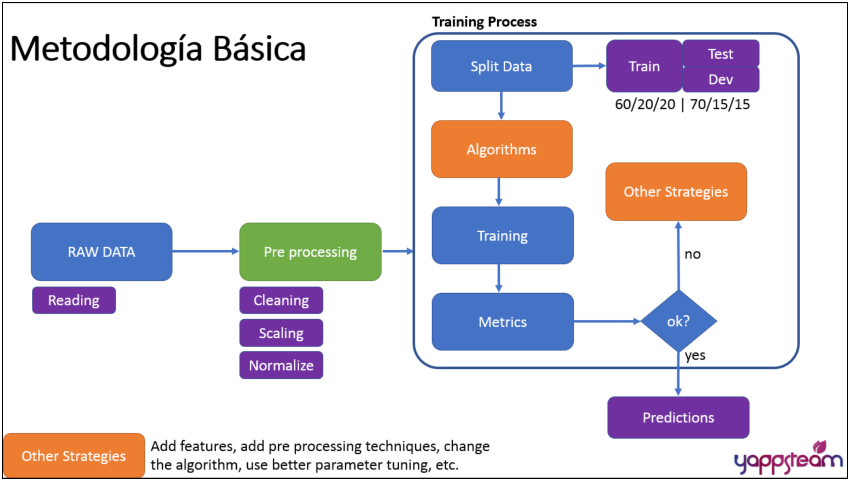
\includegraphics{./images/basic_methodology.png}
\caption{}
\end{figure}

    \section{Raw Data}\label{raw-data}

    \subsection{Reading}\label{reading}

    \begin{Verbatim}[commandchars=\\\{\}]
{\color{incolor}In [{\color{incolor}3}]:} \PY{k}{def} \PY{n+nf}{read\PYZus{}train\PYZus{}data}\PY{p}{(}\PY{p}{)}\PY{p}{:}
            \PY{l+s+sd}{\PYZsq{}\PYZsq{}\PYZsq{}Esta funcion lee los datos de entrenamiento}
        \PY{l+s+sd}{    argumentos}
        \PY{l+s+sd}{    \PYZhy{}\PYZhy{}\PYZhy{}}
        \PY{l+s+sd}{    regresa}
        \PY{l+s+sd}{    X, y \PYZhy{}\PYZhy{} datos de entrenamiento y targets}
        \PY{l+s+sd}{    \PYZsq{}\PYZsq{}\PYZsq{}}
            \PY{n}{X} \PY{o}{=} \PY{n}{pd}\PY{o}{.}\PY{n}{read\PYZus{}csv}\PY{p}{(}\PY{l+s+s1}{\PYZsq{}}\PY{l+s+s1}{./data/train\PYZus{}data.csv}\PY{l+s+s1}{\PYZsq{}}\PY{p}{,} \PY{n}{sep} \PY{o}{=} \PY{l+s+s1}{\PYZsq{}}\PY{l+s+s1}{,}\PY{l+s+s1}{\PYZsq{}}\PY{p}{)}
            \PY{n}{y} \PY{o}{=} \PY{n}{pd}\PY{o}{.}\PY{n}{read\PYZus{}csv}\PY{p}{(}\PY{l+s+s1}{\PYZsq{}}\PY{l+s+s1}{./data/y\PYZus{}train.csv}\PY{l+s+s1}{\PYZsq{}}\PY{p}{,} \PY{n}{sep} \PY{o}{=} \PY{l+s+s1}{\PYZsq{}}\PY{l+s+s1}{,}\PY{l+s+s1}{\PYZsq{}}\PY{p}{)}
            
            \PY{c+c1}{\PYZsh{} INGRESAR SU RESPUESTA DEBAJO}
            \PY{k}{return} \PY{n}{X}\PY{p}{,} \PY{n}{y} \PY{c+c1}{\PYZsh{} they should return this here}
        
        \PY{k}{def} \PY{n+nf}{read\PYZus{}test\PYZus{}data}\PY{p}{(}\PY{p}{)}\PY{p}{:}
            \PY{l+s+sd}{\PYZsq{}\PYZsq{}\PYZsq{}}
        \PY{l+s+sd}{    Esta funcion lee los datos de prueba}
        \PY{l+s+sd}{    argumentos}
        \PY{l+s+sd}{    \PYZhy{}\PYZhy{}\PYZhy{}}
        \PY{l+s+sd}{    regresa}
        \PY{l+s+sd}{    X\PYZus{}test, y\PYZus{}test \PYZhy{}\PYZhy{} datos de prueba y targets}
        \PY{l+s+sd}{    \PYZsq{}\PYZsq{}\PYZsq{}}
            \PY{n}{X\PYZus{}test} \PY{o}{=} \PY{n}{pd}\PY{o}{.}\PY{n}{read\PYZus{}csv}\PY{p}{(}\PY{l+s+s1}{\PYZsq{}}\PY{l+s+s1}{./data/test\PYZus{}data.csv}\PY{l+s+s1}{\PYZsq{}}\PY{p}{,} \PY{n}{sep} \PY{o}{=} \PY{l+s+s1}{\PYZsq{}}\PY{l+s+s1}{,}\PY{l+s+s1}{\PYZsq{}}\PY{p}{)} \PY{c+c1}{\PYZsh{}they should define X\PYZus{}test}
            \PY{n}{y\PYZus{}test} \PY{o}{=} \PY{n}{pd}\PY{o}{.}\PY{n}{read\PYZus{}csv}\PY{p}{(}\PY{l+s+s1}{\PYZsq{}}\PY{l+s+s1}{./data/y\PYZus{}test.csv}\PY{l+s+s1}{\PYZsq{}}\PY{p}{,} \PY{n}{sep} \PY{o}{=} \PY{l+s+s1}{\PYZsq{}}\PY{l+s+s1}{,}\PY{l+s+s1}{\PYZsq{}}\PY{p}{)} \PY{c+c1}{\PYZsh{}they should define y\PYZus{}test}
            
            \PY{c+c1}{\PYZsh{} INGRESAR SU RESPUESTA DEBAJO}
            \PY{k}{return} \PY{n}{X\PYZus{}test}\PY{p}{,} \PY{n}{y\PYZus{}test} \PY{c+c1}{\PYZsh{} they should return this here}
\end{Verbatim}


    \subsection{Training Data}\label{training-data}

    \begin{Verbatim}[commandchars=\\\{\}]
{\color{incolor}In [{\color{incolor}4}]:} \PY{n}{X}\PY{p}{,} \PY{n}{y} \PY{o}{=} \PY{n}{read\PYZus{}train\PYZus{}data}\PY{p}{(}\PY{p}{)} \PY{c+c1}{\PYZsh{} this must be executed}
\end{Verbatim}


    \begin{Verbatim}[commandchars=\\\{\}]
{\color{incolor}In [{\color{incolor}5}]:} \PY{n}{X}\PY{o}{.}\PY{n}{head}\PY{p}{(}\PY{l+m+mi}{7}\PY{p}{)}
\end{Verbatim}


\begin{Verbatim}[commandchars=\\\{\}]
{\color{outcolor}Out[{\color{outcolor}5}]:}       CRIM    ZN  INDUS  CHAS    NOX     RM   AGE     DIS  RAD  TAX  PTRATIO  \textbackslash{}
        0  0.24103   0.0   7.38     0  0.493  6.083  43.7  5.4159    5  287     19.6   
        1  0.09512   0.0  12.83     0  0.437  6.286  45.0  4.5026    5  398     18.7   
        2  1.61282   0.0   8.14     0  0.538  6.096  96.9  3.7598    4  307     21.0   
        3  2.14918   0.0  19.58     0  0.871  5.709  98.5  1.6232    5  403     14.7   
        4  0.02055  85.0   0.74     0  0.410  6.383  35.7  9.1876    2  313     17.3   
        5  0.08187   0.0   2.89     0  0.445  7.820  36.9  3.4952    2  276     18.0   
        6  4.75237   0.0  18.10     0  0.713  6.525  86.5  2.4358   24  666     20.2   
        
           LSTAT  
        0  12.79  
        1   8.94  
        2  20.34  
        3  15.79  
        4   5.77  
        5   3.57  
        6  18.13  
\end{Verbatim}
            
    \begin{Verbatim}[commandchars=\\\{\}]
{\color{incolor}In [{\color{incolor}6}]:} \PY{n}{X}\PY{o}{.}\PY{n}{shape}
\end{Verbatim}


\begin{Verbatim}[commandchars=\\\{\}]
{\color{outcolor}Out[{\color{outcolor}6}]:} (455, 12)
\end{Verbatim}
            
    \begin{Verbatim}[commandchars=\\\{\}]
{\color{incolor}In [{\color{incolor}7}]:} \PY{c+c1}{\PYZsh{}m, n = boston\PYZus{}data.shape}
\end{Verbatim}


    \subsection{Test Data}\label{test-data}

    \begin{Verbatim}[commandchars=\\\{\}]
{\color{incolor}In [{\color{incolor}8}]:} \PY{n}{X\PYZus{}test}\PY{p}{,} \PY{n}{y\PYZus{}test} \PY{o}{=} \PY{n}{read\PYZus{}test\PYZus{}data}\PY{p}{(}\PY{p}{)} \PY{c+c1}{\PYZsh{} this should be executed}
\end{Verbatim}


    \begin{Verbatim}[commandchars=\\\{\}]
{\color{incolor}In [{\color{incolor}9}]:} \PY{n}{X\PYZus{}test}\PY{o}{.}\PY{n}{shape}
\end{Verbatim}


\begin{Verbatim}[commandchars=\\\{\}]
{\color{outcolor}Out[{\color{outcolor}9}]:} (51, 12)
\end{Verbatim}
            
    \begin{Verbatim}[commandchars=\\\{\}]
{\color{incolor}In [{\color{incolor}10}]:} \PY{n}{X\PYZus{}test}\PY{o}{.}\PY{n}{head}\PY{p}{(}\PY{l+m+mi}{7}\PY{p}{)}
\end{Verbatim}


\begin{Verbatim}[commandchars=\\\{\}]
{\color{outcolor}Out[{\color{outcolor}10}]:}        CRIM    ZN  INDUS  CHAS    NOX     RM    AGE     DIS  RAD  TAX  \textbackslash{}
         0   0.38214   0.0   6.20     0  0.504  8.040   86.5  3.2157    8  307   
         1   0.03615  80.0   4.95     0  0.411  6.630   23.4  5.1167    4  245   
         2   0.04684   0.0   3.41     0  0.489  6.417   66.1  3.0923    2  270   
         3  11.10810   0.0  18.10     0  0.668  4.906  100.0  1.1742   24  666   
         4   0.22188  20.0   6.96     1  0.464  7.691   51.8  4.3665    3  223   
         5  25.94060   0.0  18.10     0  0.679  5.304   89.1  1.6475   24  666   
         6   0.06076   0.0  11.93     0  0.573  6.976   91.0  2.1675    1  273   
         
            PTRATIO  LSTAT  
         0     17.4   3.13  
         1     19.2   4.70  
         2     17.8   8.81  
         3     20.2  34.77  
         4     18.6   6.58  
         5     20.2  26.64  
         6     21.0   5.64  
\end{Verbatim}
            
    \begin{Verbatim}[commandchars=\\\{\}]
{\color{incolor}In [{\color{incolor}11}]:} \PY{c+c1}{\PYZsh{}m, n = boston\PYZus{}data.shape}
\end{Verbatim}


    \section{Pre Processing}\label{pre-processing}

    \begin{Verbatim}[commandchars=\\\{\}]
{\color{incolor}In [{\color{incolor}12}]:} \PY{k}{def} \PY{n+nf}{pre\PYZus{}processing}\PY{p}{(}\PY{n}{X}\PY{p}{,} \PY{n}{y}\PY{p}{)}\PY{p}{:}
             \PY{l+s+sd}{\PYZsq{}\PYZsq{}\PYZsq{}}
         \PY{l+s+sd}{    Esta fucion implementa normalizacion}
         \PY{l+s+sd}{    argumentos}
         \PY{l+s+sd}{    X \PYZhy{}\PYZhy{} datos de entrenamiento}
         \PY{l+s+sd}{    y \PYZhy{}\PYZhy{} targets}
         \PY{l+s+sd}{    }
         \PY{l+s+sd}{    regresa}
         \PY{l+s+sd}{    X\PYZus{}norm \PYZhy{}\PYZhy{} datos normalizados}
         \PY{l+s+sd}{    norm\PYZus{}data \PYZhy{}\PYZhy{} normalizador}
         \PY{l+s+sd}{    \PYZsq{}\PYZsq{}\PYZsq{}}
             \PY{n}{norm\PYZus{}data} \PY{o}{=} \PY{n}{Normalizer}\PY{p}{(}\PY{p}{)}\PY{o}{.}\PY{n}{fit}\PY{p}{(}\PY{n}{X}\PY{p}{,} \PY{n}{y}\PY{p}{)} \PY{c+c1}{\PYZsh{} this values they will be ingreseing..}
             \PY{n}{X\PYZus{}norm} \PY{o}{=} \PY{n}{norm\PYZus{}data}\PY{o}{.}\PY{n}{transform}\PY{p}{(}\PY{n}{X}\PY{p}{)}
             \PY{k}{return} \PY{n}{X\PYZus{}norm}\PY{p}{,} \PY{n}{norm\PYZus{}data} \PY{c+c1}{\PYZsh{} they should return norm\PYZus{}data| NOP THEY WONT}
\end{Verbatim}


    \begin{Verbatim}[commandchars=\\\{\}]
{\color{incolor}In [{\color{incolor}13}]:} \PY{n}{X\PYZus{}norm}\PY{p}{,} \PY{n}{norm\PYZus{}data} \PY{o}{=} \PY{n}{pre\PYZus{}processing}\PY{p}{(}\PY{n}{X}\PY{p}{,} \PY{n}{y}\PY{p}{)}
\end{Verbatim}


    Una vez que tenemos nuestros datos de entrenamiento
\textbf{normalizados}, echémosle un vistazo, para ver como difieren de
los datos de entrenamiento originales y de los datos de prueba. Para
ello usaremos \textbf{pandas}, en especifico el comando \textbf{head(n)}
nos permite visualizar los \textbf{n} primeros elementos de los datos,
en este caso vamos a usar \textbf{n = 3}.

    \begin{Verbatim}[commandchars=\\\{\}]
{\color{incolor}In [{\color{incolor}14}]:} \PY{n}{pd}\PY{o}{.}\PY{n}{DataFrame}\PY{p}{(}\PY{n}{X\PYZus{}norm}\PY{p}{)}\PY{o}{.}\PY{n}{head}\PY{p}{(}\PY{l+m+mi}{3}\PY{p}{)}
\end{Verbatim}


\begin{Verbatim}[commandchars=\\\{\}]
{\color{outcolor}Out[{\color{outcolor}14}]:}          0    1         2    3         4         5         6         7   \textbackslash{}
         0  0.000827  0.0  0.025317  0.0  0.001691  0.020868  0.149914  0.018579   
         1  0.000237  0.0  0.031964  0.0  0.001089  0.015661  0.112112  0.011218   
         2  0.004986  0.0  0.025165  0.0  0.001663  0.018846  0.299568  0.011624   
         
                  8         9         10        11  
         0  0.017153  0.984561  0.067238  0.043876  
         1  0.012457  0.991572  0.046589  0.022273  
         2  0.012366  0.949097  0.064922  0.062882  
\end{Verbatim}
            
    Bien!, ahora es tu turno, utiliza el comando \textbf{head} con un valor
\textbf{n} de \textbf{3} para visualizar los datos de entrenamiento
\textbf{X}

    \begin{Verbatim}[commandchars=\\\{\}]
{\color{incolor}In [{\color{incolor}15}]:} \PY{n}{X}\PY{o}{.}\PY{n}{head}\PY{p}{(}\PY{l+m+mi}{3}\PY{p}{)} \PY{c+c1}{\PYZsh{} they must put 3 here}
\end{Verbatim}


\begin{Verbatim}[commandchars=\\\{\}]
{\color{outcolor}Out[{\color{outcolor}15}]:}       CRIM   ZN  INDUS  CHAS    NOX     RM   AGE     DIS  RAD  TAX  PTRATIO  \textbackslash{}
         0  0.24103  0.0   7.38     0  0.493  6.083  43.7  5.4159    5  287     19.6   
         1  0.09512  0.0  12.83     0  0.437  6.286  45.0  4.5026    5  398     18.7   
         2  1.61282  0.0   8.14     0  0.538  6.096  96.9  3.7598    4  307     21.0   
         
            LSTAT  
         0  12.79  
         1   8.94  
         2  20.34  
\end{Verbatim}
            
    Ahora hagamos lo mismo con los datos de prueba \textbf{X\_test}

    \begin{Verbatim}[commandchars=\\\{\}]
{\color{incolor}In [{\color{incolor}16}]:} \PY{n}{X\PYZus{}test}\PY{o}{.}\PY{n}{head}\PY{p}{(}\PY{l+m+mi}{3}\PY{p}{)} \PY{c+c1}{\PYZsh{} they should put head(3), all the commando X\PYZus{}test.head(3)}
\end{Verbatim}


\begin{Verbatim}[commandchars=\\\{\}]
{\color{outcolor}Out[{\color{outcolor}16}]:}       CRIM    ZN  INDUS  CHAS    NOX     RM   AGE     DIS  RAD  TAX  PTRATIO  \textbackslash{}
         0  0.38214   0.0   6.20     0  0.504  8.040  86.5  3.2157    8  307     17.4   
         1  0.03615  80.0   4.95     0  0.411  6.630  23.4  5.1167    4  245     19.2   
         2  0.04684   0.0   3.41     0  0.489  6.417  66.1  3.0923    2  270     17.8   
         
            LSTAT  
         0   3.13  
         1   4.70  
         2   8.81  
\end{Verbatim}
            
    \section{Training Process}\label{training-process}

    \subsection{Split Data}\label{split-data}

    Ya hemos cargando nuestros datos de entrenamiento y prueba (test)
respectivamente, no obstante aun necesitamos aplicar la normalización a
nuestros datos de prueba, eso lo podemos realizar usando el objeto
\textbf{norm\_data} que obtuvimos en el proceso de normalización, para
ello simplemente tenemos que pasar los datos de prueba \textbf{X\_test}

    \begin{Verbatim}[commandchars=\\\{\}]
{\color{incolor}In [{\color{incolor}17}]:} \PY{n}{X\PYZus{}test\PYZus{}norm} \PY{o}{=} \PY{n}{norm\PYZus{}data}\PY{o}{.}\PY{n}{transform}\PY{p}{(}\PY{n}{X\PYZus{}test}\PY{p}{)}
\end{Verbatim}


    Antes de proceder comparemos los datos de prueba \textbf{X\_test} con su
versión normalizada \textbf{X\_test\_norm}, para ello usaremos
nuevamente el comando \textbf{head(n)}, recuerda usar \textbf{n = 3}

    \begin{Verbatim}[commandchars=\\\{\}]
{\color{incolor}In [{\color{incolor}18}]:} \PY{n}{pd}\PY{o}{.}\PY{n}{DataFrame}\PY{p}{(}\PY{n}{X\PYZus{}test\PYZus{}norm}\PY{p}{)}\PY{o}{.}\PY{n}{head}\PY{p}{(}\PY{l+m+mi}{3}\PY{p}{)}
\end{Verbatim}


\begin{Verbatim}[commandchars=\\\{\}]
{\color{outcolor}Out[{\color{outcolor}18}]:}          0         1         2    3         4         5         6         7   \textbackslash{}
         0  0.001195  0.000000  0.019392  0.0  0.001576  0.025147  0.270548  0.010058   
         1  0.000139  0.307979  0.019056  0.0  0.001582  0.025524  0.090084  0.019698   
         2  0.000168  0.000000  0.012231  0.0  0.001754  0.023016  0.237086  0.011091   
         
                  8         9         10        11  
         0  0.025022  0.960212  0.054422  0.009790  
         1  0.015399  0.943186  0.073915  0.018094  
         2  0.007174  0.968431  0.063845  0.031600  
\end{Verbatim}
            
    \begin{Verbatim}[commandchars=\\\{\}]
{\color{incolor}In [{\color{incolor}19}]:} \PY{n}{X\PYZus{}test}\PY{o}{.}\PY{n}{head}\PY{p}{(}\PY{l+m+mi}{3}\PY{p}{)}
\end{Verbatim}


\begin{Verbatim}[commandchars=\\\{\}]
{\color{outcolor}Out[{\color{outcolor}19}]:}       CRIM    ZN  INDUS  CHAS    NOX     RM   AGE     DIS  RAD  TAX  PTRATIO  \textbackslash{}
         0  0.38214   0.0   6.20     0  0.504  8.040  86.5  3.2157    8  307     17.4   
         1  0.03615  80.0   4.95     0  0.411  6.630  23.4  5.1167    4  245     19.2   
         2  0.04684   0.0   3.41     0  0.489  6.417  66.1  3.0923    2  270     17.8   
         
            LSTAT  
         0   3.13  
         1   4.70  
         2   8.81  
\end{Verbatim}
            
    Excelente, como podrás notar, los datos normalizados difieren de los
datos originales, ya sea en su versión de entrenamiento o prueba, esto
se debe a que la normalización \textbf{"centra"} los datos, es decir
trata de encontrar el valor en el que se encuentra distribuidos los
datos.

    \subsection{Algorithms}\label{algorithms}

    El modelo que usaremos es el descrito en las diapositivas, el cual
recibe el nombre de regresión lineal, como vimos, este modelo puede ser
aplicado no solo a 1 dimensión, sino que se puede generalizar a varias
dimensiones de la siguiente manera:

    \begin{figure}
\centering
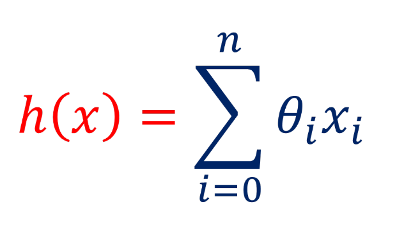
\includegraphics{./images/model.png}
\caption{model}
\end{figure}

    Para definir nuestro modelo seguiremos los siguientes pasos: 1. Primero
crearemos una función llamada \textbf{linear\_regression}

\begin{verbatim}
```python
def linear_regression():
```
\end{verbatim}

\begin{enumerate}
\def\labelenumi{\arabic{enumi}.}
\setcounter{enumi}{1}
\item
  Como hemos visto hasta ahora, para que nuestro modelo pueda aprender
  necesitamos los datos de entrenamiento \textbf{X} y los targets
  \textbf{y}, por ende estos serán las entradas de nuestra función
  \textbf{linear\_regression}

\begin{Shaded}
\begin{Highlighting}[]
\KeywordTok{def}\NormalTok{ linear_regression(X, y):}
\end{Highlighting}
\end{Shaded}
\item
  Ahora usaremos una variable para definir nuestro modelo llamada
  \textbf{model}

\begin{Shaded}
\begin{Highlighting}[]
\KeywordTok{def}\NormalTok{ linear_regression(X, y):}
\NormalTok{     model }\OperatorTok{=}\NormalTok{ ...}
\end{Highlighting}
\end{Shaded}
\item
  Usando el comando \textbf{LinearRegression()} podemos crear el modelo

\begin{Shaded}
\begin{Highlighting}[]
\KeywordTok{def}\NormalTok{ linear_regression(X, y):}
\NormalTok{     model }\OperatorTok{=}\NormalTok{ LinearRegression()}
\end{Highlighting}
\end{Shaded}
\item
  Debemos definir que hiper-parámetros se usaran; en el caso del modelo
  de regresión lineal usaremos: \textbf{normalize = True} y
  \textbf{fit\_intercept = True}.

\begin{Shaded}
\begin{Highlighting}[]
\KeywordTok{def}\NormalTok{ linear_regression(X, y):}
\NormalTok{     model }\OperatorTok{=}\NormalTok{ LinearRegression(normalize }\OperatorTok{=} \VariableTok{True}\NormalTok{, fit_intercept }\OperatorTok{=} \VariableTok{True}\NormalTok{)}
\end{Highlighting}
\end{Shaded}
\item
  Una vez hecho eso, podemos entrenar nuestro modelo, para ello usaremos
  el comando \textbf{fit}, el cual recibirá los datos de entrenamiento
  \textbf{X} y targets \textbf{y}

\begin{Shaded}
\begin{Highlighting}[]
\KeywordTok{def}\NormalTok{ linear_regression(X, y):}
\NormalTok{     model }\OperatorTok{=}\NormalTok{ LinearRegression(normalize }\OperatorTok{=} \VariableTok{True}\NormalTok{, fit_intercept }\OperatorTok{=} \VariableTok{True}\NormalTok{)}
\NormalTok{     model.fit(X, y)}
\end{Highlighting}
\end{Shaded}
\item
  Finalmente retornamos nuestro modelo entrenado
  \texttt{python\ def\ linear\_regression(X,\ y):\ \ \ \ \ \ model\ =\ LinearRegression(normalize\ =\ True,\ fit\_intercept\ =\ True)\ \ \ \ \ \ model.fit(X,\ y)\ \ \ \ \ \ return\ ...}
\end{enumerate}

    \begin{Verbatim}[commandchars=\\\{\}]
{\color{incolor}In [{\color{incolor}20}]:} \PY{c+c1}{\PYZsh{} def linear\PYZus{}regression():}
         \PY{k}{def} \PY{n+nf}{linear\PYZus{}regression}\PY{p}{(}\PY{n}{X}\PY{p}{,} \PY{n}{y}\PY{p}{)}\PY{p}{:} \PY{c+c1}{\PYZsh{} X, y must have been ingresed}
             \PY{l+s+sd}{\PYZsq{}\PYZsq{}\PYZsq{}}
         \PY{l+s+sd}{    Esta funcion crea y entrena un modelo de regresion lineal}
         \PY{l+s+sd}{    argumentos}
         \PY{l+s+sd}{    X, y \PYZhy{}\PYZhy{} datos de entrenamiento y targets}
         \PY{l+s+sd}{    regresa}
         \PY{l+s+sd}{    model \PYZhy{}\PYZhy{} modelo de regresion lineal entrenado}
         \PY{l+s+sd}{    \PYZsq{}\PYZsq{}\PYZsq{}}
             \PY{n}{model} \PY{o}{=} \PY{o}{.}\PY{o}{.}\PY{o}{.}
             \PY{n}{model} \PY{o}{=} \PY{n}{LinearRegression}\PY{p}{(}\PY{n}{normalize} \PY{o}{=} \PY{k+kc}{True}\PY{p}{,} \PY{n}{fit\PYZus{}intercept} \PY{o}{=} \PY{k+kc}{True}\PY{p}{)} \PY{c+c1}{\PYZsh{} they should define the model [True, both]}
             \PY{c+c1}{\PYZsh{} Training}
             \PY{n+nb}{print}\PY{p}{(}\PY{l+s+s1}{\PYZsq{}}\PY{l+s+s1}{Entrenamiento Iniciado}\PY{l+s+s1}{\PYZsq{}}\PY{p}{)}
             \PY{n}{model}\PY{o}{.}\PY{n}{fit}\PY{p}{(}\PY{n}{X}\PY{p}{,} \PY{n}{y}\PY{p}{)} \PY{c+c1}{\PYZsh{} they also should define X, y}
             \PY{n+nb}{print}\PY{p}{(}\PY{l+s+s1}{\PYZsq{}}\PY{l+s+s1}{Entrenamiento Completado}\PY{l+s+s1}{\PYZsq{}}\PY{p}{)}
             \PY{k}{return} \PY{n}{model} \PY{c+c1}{\PYZsh{} they must return the model}
\end{Verbatim}


    \subsection{Training}\label{training}

    Hora de entrenar nuestro modelo, en este caso vamos a entrenar dos
modelos, uno de ellos se entrenara con los datos normalizados y el otro
con los datos sin normalizar, recuerda que la \textbf{función
linear\_regression(X, y)} que hemos definido toma dos argumentos, los
datos \textbf{X} y los targets \textbf{y}.

    \begin{Verbatim}[commandchars=\\\{\}]
{\color{incolor}In [{\color{incolor}21}]:} \PY{c+c1}{\PYZsh{} Este modelo usara los datos normalizados X\PYZus{}norm}
         \PY{n}{modelo1} \PY{o}{=} \PY{n}{linear\PYZus{}regression}\PY{p}{(}\PY{n}{X\PYZus{}norm}\PY{p}{,} \PY{n}{y}\PY{p}{)}
         \PY{c+c1}{\PYZsh{} Y el segundo modelo usara los datos sin normalizar X}
         \PY{n}{modelo2} \PY{o}{=} \PY{n}{linear\PYZus{}regression}\PY{p}{(}\PY{n}{X}\PY{p}{,} \PY{n}{y}\PY{p}{)}
\end{Verbatim}


    \begin{Verbatim}[commandchars=\\\{\}]
Entrenamiento Iniciado
Entrenamiento Completado
Entrenamiento Iniciado
Entrenamiento Completado

    \end{Verbatim}

    \subsection{Predictions}\label{predictions}

    Felicidades!, ya has entrenado dos modelos!!, ahora, que tal si hacemos
algunas predicciones, para ello debemos recordar que, los modelos
necesitan los datos \textbf{X} y \textbf{X\_norm} respectivamente para
poder realizar predicciones; estos datos los usaremos de la siguiente
manera: \textbf{\emph{modelo1.predict(...)}}. A las predicciones les
denominaremos \textbf{y\_hat}, como tenemos dos modelos, usaremos
\textbf{y\_hat\_norm} para referirnos al modelo que usa los datos
normalizados y \textbf{y\_hat} para el modelo que usa los datos
\textbf{X}

    \subsubsection{Training}\label{training}

    Comencemos con los datos de entrenamiento, para ello usaremos
\textbf{\emph{modelo1.predict(X)}} para los resultados de
\textbf{y\_hat}, ya que este modelo se entreno usando los datos
originales \textbf{X}, y para \textbf{y\_hat\_norm} usaremos
\textbf{\emph{modelo1.predict(X\_norm)}}

    \begin{Verbatim}[commandchars=\\\{\}]
{\color{incolor}In [{\color{incolor}22}]:} \PY{n}{y\PYZus{}hat} \PY{o}{=} \PY{n}{modelo2}\PY{o}{.}\PY{n}{predict}\PY{p}{(}\PY{n}{X}\PY{p}{)}
         \PY{n}{y\PYZus{}hat\PYZus{}norm} \PY{o}{=} \PY{n}{modelo1}\PY{o}{.}\PY{n}{predict}\PY{p}{(}\PY{n}{X\PYZus{}norm}\PY{p}{)}
\end{Verbatim}


    Ahora echemos un vistazo a lo que nuestros modelos predicen!!

    \begin{Verbatim}[commandchars=\\\{\}]
{\color{incolor}In [{\color{incolor}23}]:} \PY{n}{results\PYZus{}training} \PY{o}{=} \PY{n}{result\PYZus{}table}\PY{p}{(}\PY{n}{y}\PY{p}{,} \PY{n}{y\PYZus{}hat}\PY{p}{,} \PY{n}{y\PYZus{}hat\PYZus{}norm}\PY{p}{)}
         \PY{n}{results\PYZus{}training}\PY{o}{.}\PY{n}{head}\PY{p}{(}\PY{l+m+mi}{7}\PY{p}{)}
\end{Verbatim}


\begin{Verbatim}[commandchars=\\\{\}]
{\color{outcolor}Out[{\color{outcolor}23}]:}    valores y originales      y\_hat  y\_hat\_norm
         0                  22.2  19.062556   18.804516
         1                  21.4  23.876561   23.996453
         2                  13.5  14.276546   14.456355
         3                  19.4  17.902439   17.751349
         4                  24.7  25.084858   24.209114
         5                  43.8  35.226664   38.874021
         6                  14.1  17.916197   19.099431
\end{Verbatim}
            
    \textbf{Pregunta de Taller:} Que observaciones puedes notar?

    \subsubsection{Test}\label{test}

    Ahora hagamos lo mismo con los datos de prueba, para ello usaremos
\textbf{X\_test} para \textbf{y\_hat} y \textbf{X\_test\_norm} para
\textbf{y\_hat\_norm}

    \begin{Verbatim}[commandchars=\\\{\}]
{\color{incolor}In [{\color{incolor}24}]:} \PY{n}{y\PYZus{}hat} \PY{o}{=} \PY{n}{modelo2}\PY{o}{.}\PY{n}{predict}\PY{p}{(}\PY{n}{X\PYZus{}test}\PY{p}{)} \PY{c+c1}{\PYZsh{} ellos llenan aqui}
         \PY{n}{y\PYZus{}hat\PYZus{}norm} \PY{o}{=} \PY{n}{modelo1}\PY{o}{.}\PY{n}{predict}\PY{p}{(}\PY{n}{X\PYZus{}test\PYZus{}norm}\PY{p}{)} \PY{c+c1}{\PYZsh{} y aqui}
\end{Verbatim}


    Veamos los resultados

    \begin{Verbatim}[commandchars=\\\{\}]
{\color{incolor}In [{\color{incolor}25}]:} \PY{n}{results\PYZus{}test} \PY{o}{=} \PY{n}{result\PYZus{}table}\PY{p}{(}\PY{n}{y\PYZus{}test}\PY{p}{,} \PY{n}{y\PYZus{}hat}\PY{p}{,} \PY{n}{y\PYZus{}hat\PYZus{}norm}\PY{p}{)}
         \PY{n}{results\PYZus{}test}\PY{o}{.}\PY{n}{head}\PY{p}{(}\PY{l+m+mi}{7}\PY{p}{)}
\end{Verbatim}


\begin{Verbatim}[commandchars=\\\{\}]
{\color{outcolor}Out[{\color{outcolor}25}]:}    valores y originales      y\_hat  y\_hat\_norm
         0                  37.6  38.065522   38.695965
         1                  27.9  32.012522   30.307269
         2                  22.6  27.220585   26.767393
         3                  13.8   3.500439   10.134246
         4                  35.2  35.868174   40.829790
         5                  10.4   7.284909   10.206643
         6                  23.9  28.092602   29.118654
\end{Verbatim}
            
    \textbf{Pregunta de Taller:} Que observaciones puedes notar?

    \subsection{Metrics}\label{metrics}

    Como vimos en la definición de machine learning, necesitamos de una
forma de medir que tanto nuestro modelo ha aprendido, para ello existen
las métricas de evaluación, estas nos permiten determinar dos aspectos
fundamentales:

\begin{itemize}
\tightlist
\item
  El nivel de exactitud del modelo
\item
  El nivel de error
\end{itemize}

En esta oportunidad estaremos usando la métrica \textbf{r score}, esta
define de la siguiente manera:

    \begin{figure}
\centering
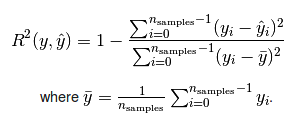
\includegraphics{./images/r2_score.png}
\caption{r2\_score}
\end{figure}

    Ahora vamos a usar esta formula, para ello usaremos la \textbf{función
r2\_score}, esta función toma dos valores: * y: Los targets originales *
y\_hat: Los targets que predice nuestro modelo Primero vamos a calcular
\textbf{y\_hat}, para ello usaremos la variable \textbf{y\_hat\_tr} para
referirnos a los resultados de los datos de entrenamiento sin
normalización y \textbf{y\_hat\_tr\_norm} con normalización
respectivamente.

    \subsubsection{Training}\label{training}

    \begin{Verbatim}[commandchars=\\\{\}]
{\color{incolor}In [{\color{incolor}26}]:} \PY{n}{y\PYZus{}hat\PYZus{}tr\PYZus{}norm}\PY{o}{=} \PY{n}{modelo1}\PY{o}{.}\PY{n}{predict}\PY{p}{(}\PY{n}{X\PYZus{}norm}\PY{p}{)}
         \PY{n}{y\PYZus{}hat\PYZus{}tr} \PY{o}{=} \PY{n}{modelo2}\PY{o}{.}\PY{n}{predict}\PY{p}{(}\PY{n}{X}\PY{p}{)}
\end{Verbatim}


    \subsubsection{Test}\label{test}

Ahora procederemos con los datos de prueba, para ello usaremos
\textbf{y\_hat\_ts} sin normalización y \textbf{y\_hat\_ts\_norm} con
normalización

    \begin{Verbatim}[commandchars=\\\{\}]
{\color{incolor}In [{\color{incolor}27}]:} \PY{n}{y\PYZus{}hat\PYZus{}ts\PYZus{}norm} \PY{o}{=} \PY{n}{modelo1}\PY{o}{.}\PY{n}{predict}\PY{p}{(}\PY{n}{X\PYZus{}test\PYZus{}norm}\PY{p}{)}
         \PY{n}{y\PYZus{}hat\PYZus{}ts} \PY{o}{=} \PY{n}{modelo2}\PY{o}{.}\PY{n}{predict}\PY{p}{(}\PY{n}{X\PYZus{}test}\PY{p}{)}
\end{Verbatim}


    Ahora aplicaremos \textbf{r score}, recuerda que ya hemos calculado
\textbf{y} e \textbf{y\_hat}

    \subsubsection{Training Metrics}\label{training-metrics}

    Nuestro modelo con normalización en los datos de entrenamiento obtiene
un aproximado de \textbf{0.72\%} de puntaje

    \begin{Verbatim}[commandchars=\\\{\}]
{\color{incolor}In [{\color{incolor}28}]:} \PY{n}{r2\PYZus{}score}\PY{p}{(}\PY{n}{y}\PY{p}{,} \PY{n}{y\PYZus{}hat\PYZus{}tr\PYZus{}norm}\PY{p}{)}
\end{Verbatim}


\begin{Verbatim}[commandchars=\\\{\}]
{\color{outcolor}Out[{\color{outcolor}28}]:} 0.7229693210852297
\end{Verbatim}
            
    Mientras que el modelo sin normalización en los datos de entrenamiento
obtiene un aproximado de \textbf{0.73\%} de puntaje

    \begin{Verbatim}[commandchars=\\\{\}]
{\color{incolor}In [{\color{incolor}29}]:} \PY{n}{r2\PYZus{}score}\PY{p}{(}\PY{n}{y}\PY{p}{,} \PY{n}{y\PYZus{}hat\PYZus{}tr}\PY{p}{)}
\end{Verbatim}


\begin{Verbatim}[commandchars=\\\{\}]
{\color{outcolor}Out[{\color{outcolor}29}]:} 0.733123926171427
\end{Verbatim}
            
    \textbf{Pregunta de Taller:} Que observaciones puedes notar?

    \subsubsection{Test Metrics}\label{test-metrics}

    No obstante en los datos de prueba el modelo con normalización obtiene
\textbf{0.83\%} de puntaje

    \begin{Verbatim}[commandchars=\\\{\}]
{\color{incolor}In [{\color{incolor}30}]:} \PY{n}{r2\PYZus{}score}\PY{p}{(}\PY{n}{y\PYZus{}test}\PY{p}{,} \PY{n}{y\PYZus{}hat\PYZus{}ts\PYZus{}norm}\PY{p}{)}
\end{Verbatim}


\begin{Verbatim}[commandchars=\\\{\}]
{\color{outcolor}Out[{\color{outcolor}30}]:} 0.8293030922289955
\end{Verbatim}
            
    Mientras que nuestro modelo sin normalización solo obtiene un
\textbf{0.72\%} de puntaje

    \begin{Verbatim}[commandchars=\\\{\}]
{\color{incolor}In [{\color{incolor}31}]:} \PY{n}{r2\PYZus{}score}\PY{p}{(}\PY{n}{y\PYZus{}test}\PY{p}{,} \PY{n}{y\PYZus{}hat\PYZus{}ts}\PY{p}{)}
\end{Verbatim}


\begin{Verbatim}[commandchars=\\\{\}]
{\color{outcolor}Out[{\color{outcolor}31}]:} 0.7184173788848401
\end{Verbatim}
            
    \begin{longtable}[]{@{}lll@{}}
\toprule
Modelo & Datos & r score\tabularnewline
\midrule
\endhead
Modelo 1 & Entrenamiento & 0.72\tabularnewline
Modelo 2 & Entrenamiento & \textbf{0.73}\tabularnewline
Modelo 1 & Prueba & \textbf{0.83}\tabularnewline
Modelo 2 & Prueba & 0.72\tabularnewline
\bottomrule
\end{longtable}

    \textbf{Pregunta de Taller:} Que observaciones puedes notar?

    \section{Visualizations}\label{visualizations}

    Buen trabajo, ya hemos entrenado y validado nuestro modelo, no obstante
aun podemos hacer mas!, en esta sección analizaremos los resultados
obtenidos desde una perspectiva mas grafica.

    \subsubsection{Training}\label{training}

    Ejecuta la siguiente celda para visualizar los resultados en los datos
de entrenamiento

    \begin{Verbatim}[commandchars=\\\{\}]
{\color{incolor}In [{\color{incolor}32}]:} \PY{n}{plot\PYZus{}data\PYZus{}train} \PY{o}{=} \PY{n}{plot\PYZus{}data\PYZus{}results}\PY{p}{(}\PY{n}{y\PYZus{}hat\PYZus{}tr\PYZus{}norm}\PY{p}{,} \PY{n}{y\PYZus{}hat\PYZus{}tr}\PY{p}{,} \PY{n}{y}\PY{p}{)}
         \PY{n}{sea}\PY{o}{.}\PY{n}{lmplot}\PY{p}{(}\PY{n}{x} \PY{o}{=} \PY{l+s+s1}{\PYZsq{}}\PY{l+s+s1}{y\PYZus{}test}\PY{l+s+s1}{\PYZsq{}}\PY{p}{,} \PY{n}{y} \PY{o}{=} \PY{l+s+s1}{\PYZsq{}}\PY{l+s+s1}{y\PYZus{}hat}\PY{l+s+s1}{\PYZsq{}}\PY{p}{,} \PY{n}{data} \PY{o}{=} \PY{n}{plot\PYZus{}data\PYZus{}train}\PY{p}{,} \PY{n}{fit\PYZus{}reg} \PY{o}{=} \PY{k+kc}{False}\PY{p}{,} \PY{n}{size} \PY{o}{=} \PY{l+m+mi}{7}\PY{p}{,} \PY{n}{col} \PY{o}{=} \PY{l+s+s1}{\PYZsq{}}\PY{l+s+s1}{modelo}\PY{l+s+s1}{\PYZsq{}}\PY{p}{)}
\end{Verbatim}


\begin{Verbatim}[commandchars=\\\{\}]
{\color{outcolor}Out[{\color{outcolor}32}]:} <seaborn.axisgrid.FacetGrid at 0x7f4d9925b5c0>
\end{Verbatim}
            
    \begin{center}
    \adjustimage{max size={0.9\linewidth}{0.9\paperheight}}{output_93_1.png}
    \end{center}
    { \hspace*{\fill} \\}
    
    \subsubsection{Test}\label{test}

    Ahora hagamos lo mismo con los datos de prueba.

    \begin{Verbatim}[commandchars=\\\{\}]
{\color{incolor}In [{\color{incolor}33}]:} \PY{n}{plot\PYZus{}data\PYZus{}test} \PY{o}{=} \PY{n}{plot\PYZus{}data\PYZus{}results}\PY{p}{(}\PY{n}{y\PYZus{}hat\PYZus{}ts\PYZus{}norm}\PY{p}{,} \PY{n}{y\PYZus{}hat\PYZus{}ts}\PY{p}{,} \PY{n}{y\PYZus{}test}\PY{p}{)}
         \PY{n}{sea}\PY{o}{.}\PY{n}{lmplot}\PY{p}{(}\PY{n}{x} \PY{o}{=} \PY{l+s+s1}{\PYZsq{}}\PY{l+s+s1}{y\PYZus{}test}\PY{l+s+s1}{\PYZsq{}}\PY{p}{,} \PY{n}{y} \PY{o}{=} \PY{l+s+s1}{\PYZsq{}}\PY{l+s+s1}{y\PYZus{}hat}\PY{l+s+s1}{\PYZsq{}}\PY{p}{,} \PY{n}{data} \PY{o}{=} \PY{n}{plot\PYZus{}data\PYZus{}test}\PY{p}{,} \PY{n}{fit\PYZus{}reg} \PY{o}{=} \PY{k+kc}{False}\PY{p}{,} \PY{n}{size} \PY{o}{=} \PY{l+m+mi}{7}\PY{p}{,} \PY{n}{col} \PY{o}{=} \PY{l+s+s1}{\PYZsq{}}\PY{l+s+s1}{modelo}\PY{l+s+s1}{\PYZsq{}}\PY{p}{)}
\end{Verbatim}


\begin{Verbatim}[commandchars=\\\{\}]
{\color{outcolor}Out[{\color{outcolor}33}]:} <seaborn.axisgrid.FacetGrid at 0x7f4d992c7080>
\end{Verbatim}
            
    \begin{center}
    \adjustimage{max size={0.9\linewidth}{0.9\paperheight}}{output_96_1.png}
    \end{center}
    { \hspace*{\fill} \\}
    
    Perfecto, ya tenemos nuestras visualizaciones, ahora que tal si echamos
un vistazo a los \textbf{coeficientes} de nuestros modelos.

    \begin{Verbatim}[commandchars=\\\{\}]
{\color{incolor}In [{\color{incolor}34}]:} \PY{n}{coef\PYZus{}data} \PY{o}{=} \PY{n}{coef\PYZus{}info}\PY{p}{(}\PY{n+nb}{list}\PY{p}{(}\PY{n}{X}\PY{o}{.}\PY{n}{columns}\PY{p}{)}\PY{p}{,} \PY{n}{modelo1}\PY{o}{.}\PY{n}{coef\PYZus{}}\PY{o}{.}\PY{n}{T}\PY{p}{,} \PY{n}{modelo2}\PY{o}{.}\PY{n}{coef\PYZus{}}\PY{o}{.}\PY{n}{T}\PY{p}{)}
         \PY{n}{coef\PYZus{}data}
\end{Verbatim}


\begin{Verbatim}[commandchars=\\\{\}]
{\color{outcolor}Out[{\color{outcolor}34}]:}    features  coef\_modelo1  coef\_modelo2
         0      CRIM   -131.447736     -0.123935
         1        ZN    -16.362026      0.044587
         2     INDUS      8.422557      0.010337
         3      CHAS    952.353670      3.056300
         4       NOX  -4469.143310    -17.208721
         5        RM   1737.061185      3.556852
         6       AGE    -20.412338      0.007283
         7       DIS   -226.668674     -1.429157
         8       RAD     27.132901      0.318979
         9       TAX   -108.077815     -0.013684
         10  PTRATIO   -294.512115     -0.909064
         11    LSTAT   -174.694457     -0.633729
\end{Verbatim}
            
    \subsection{Conclusiones}\label{conclusiones}

Buen trabajo, has entrenado tu primer modelo de \textbf{Machine
Learning} :), aquí hay unas cuantas cosas que son importantes recordar:
* El objetivo de Machine Learning es la creación de algoritmos (modelos)
que puedan aprender de los datos (como hemos visto en este Taller). * El
algoritmo de regresión lineal que has implementado es capaz de predecir
exitosamente los precios de los inmuebles, gracias a que le has brindado
datos \textbf{X} y \textbf{y} de donde aprenda. * Las métricas son
usadas para evaluar que tanto nuestros algoritmos (modelos) han
aprendido. * Si bien es cierto las métricas son importantes, usando
gráficos podemos obtener información mas detallada acerca de los
resultados que obtenemos.

Finalmente, gracias por haber estado presente el día de hoy, esperamos
que este Taller haya sido de tu agrado, no olvides visitar
(\textbf{yappsteam}){[}https://www.facebook.com/yappsteam/{]} en
Facebook para enterarte de mas novedades :D

    \begin{Verbatim}[commandchars=\\\{\}]
{\color{incolor}In [{\color{incolor} }]:} \PY{c+c1}{\PYZsh{} Viernes 27 de abril}
        \PY{c+c1}{\PYZsh{} aula: G 601}
        \PY{c+c1}{\PYZsh{} hora: 3 \PYZti{} 6pm}
\end{Verbatim}



    % Add a bibliography block to the postdoc
    
    
    
    \end{document}
